\documentclass[aps,prb,twocolumn,superscriptaddress,floatfix,longbibliography,citeautoscript]{revtex4-2}

% Conveniently, the citeautoscript option in the revtex4-2 class toggles the spacing & punctuation automatically for superscript vs. bracketed citations. Place citations as if they were in [].
% Uncomment the line below to do superscript citations.
% \setcitestyle{super}

\usepackage{amsmath,amssymb} % math symbols
\usepackage{bm} % bold math font
\usepackage{graphicx} % for figures
\usepackage{comment} % allows block comments
\usepackage[normalem]{ulem} % allows strikeout text, e.g. \sout{text}

% \usepackage{minted} % allows colored code
% \usepackage{textcomp} % This package gives the text quote '

\usepackage{enumitem}
\setlist{noitemsep,leftmargin=*,topsep=0pt,parsep=0pt}

\usepackage{xcolor} % \textcolor{red}{text} will be red for notes
\definecolor{lightgray}{gray}{0.6}
\definecolor{medgray}{gray}{0.4}
\definecolor{mRed}{RGB}{230, 0, 50}
\colorlet{newtextColor}{mRed}

\usepackage{hyperref}
\hypersetup{
colorlinks=true,
urlcolor= blue,
citecolor=blue,
linkcolor= blue,
}

% Code to add paragraph numbers and titles
\newif\ifptitle
\newif\ifpnumber
\newcounter{para}
\newcommand\ptitle[1]{\par\refstepcounter{para}
{\ifpnumber{\noindent\textcolor{lightgray}{\textbf{\thepara}}\indent}\fi}
{\ifptitle{\textbf{[{#1}]}}\fi}}
%\ptitletrue  % comment this line to hide paragraph titles
%\pnumbertrue  % comment this line to hide paragraph numbers

% Code for reviewer text
%\newcommand{\revtext}[1]{\textcolor{reviewColor}{#1}}
\newcommand{\revtext}[1]{\textit{#1}}

% Code to track changes
\newif\iftrackchanges
\newcommand{\newtext}[1]
    {\textcolor{\iftrackchanges newtextColor\else black\fi}{#1}}
\newcommand{\deltext}[1]
    {\iftrackchanges{\textcolor{newtextColor}{\sout{#1}}}\fi}
%\trackchangestrue  % comment to hide tracked changes

% Instead of making TONS of colored newtext, let's just put a colored line next to big blocks of new text.
\usepackage{mdframed}
\newmdenv[
  linecolor={\iftrackchanges newtextColor\else white\fi},
  linewidth=2pt,
  topline=false,
  bottomline=false,
  rightline=false,
  skipabove=\topsep,
  skipbelow=\topsep,
  leftmargin=-12pt,
  innertopmargin=0pt,
  innerbottommargin=0pt
]{newtextblock}

% Uncomment this line if you prefer your vectors to appear as bold letters.
% By default they will appear with arrows over them.
% \renewcommand{\vec}[1]{\bm{#1}}

% Command to mark text in blue/red and define common units
\newcommand{\blue}[1]{\textcolor{blue}{#1}}
\newcommand{\red}[1]{\textcolor{red}{#1}}
\newcommand{\df}[1]{\dfrac}
\newcommand{\mic}{\mu\mathrm{m}}
\newcommand{\nm}{\mathrm{nm}}
\newcommand{\mm}{\mathrm{mm}}
\newcommand{\mrm}[1]{\mathrm{#1}}
\newcommand{\la}{\langle}
\newcommand{\ra}{\rangle}

\ptitletrue
\pnumbertrue

% Replace minted with listings if you don't want to install Pygments
\usepackage{listings}
\usepackage{graphicx}
\usepackage{float}
% minimum font size for figures
\newcommand{\minfont}{6}

% Author affiliations
\newcommand{\heng}{School of Engineering \& Applied Sciences, Harvard University, Cambridge, Massachusetts 02138, USA}
\newcommand{\hphys}{Department of Physics, Harvard University, Cambridge, Massachusetts 02138, USA}

% Allows rewriting the same title in the supplement
\newcommand{\mytitle}{Optical Tweezer Experiment Outline}

\begin{document}

\title{\mytitle}

\author{Adam Pearl}
\email[]{apearl@college.harvard.edu}
\affiliation{\hphys}
\author{Nicholas Lyu}
\email[]{nicholaslyu@college.harvard.edu}
\affiliation{\hphys}
% \affiliation{\heng}

\date{\today}

\begin{abstract}
This paper outlines the design, alignment, and calibration of a single-beam optical tweezer apparatus. 
We aim to trap dielectric spheres in solution and measure the trap depth. 
\end{abstract}

\maketitle

%%%%%%%%%%%%%%%%%%%%%%%%%%%%%%%%%%%%%%%%%%%%%%%%%%%%%%%%%%%%%%%%%%%%%%%%
\section{\label{sec:intro}Introduction}
 We introduce the two goals of our experiment: to measure the muon's lifetime and mass. We give a brief historical background to the original experiments that measured these quantities and provide the current accepted PDG values for each.

%%%%%%%%%%%%%%%%%%%%%%%%%%%%%%%%%%%%%%%%%%%%%%%%%%%%%%%%%%%%%%%%%%%%%%%%
\section{\label{sec:theory}Theory and Background}

In this section, we give a high-level explanation of the nuclear processes that we care about in this experiment. We want to discuss the decays of kaons and pions in cosmic rays to muons and the subsequent decays to electrons and neutrinos.
\subsection{Lifetime}

We motivate the exponential decay of the muon and explain how we extract the lifetime by fitting the exponential decay.

\subsection{Mass}
We explain the muon to electron and neutrino decay and motivate the assumption that the muon decays at rest. We show that we can measure the mass of the muon by measuring the maximum energy of the electron

We look for events that pass through our top and middle detectors but not our bottom detector

We explain why we measure the maximal electron energy (electrons can lose energy, we want to measure the electron with the least energy loss).

\section{\label{sec:methods}Methods}
\subsection{Fitting and background correction}
We explain how we fit the logarithmic decay curve, including our assumption of constant background and how we corrected for it, and our method for determining the optimal hyperparameters (clipping data and bin width).
\subsection{Electron pulse calibration}
We need to explain the concept of minimally ionizing particles (MIPS). We make the educated assumption that muons that pass through all three detectors are minimally ionizing. The Bethe Bloche equation gives the average rate of ionizing energy loss per unit distance, $-\langle \frac{dE}{dx}\rangle$ as a function of the relativistic \blue{what is it called} $\beta\gamma$. Using the thickness of the detector, we can estimate $E$ for a MIP. We trigger on $TMB$ and measure the average electron pulse height. We compare this to the $E$ to get a conversion from pulse amplitude (voltage) to energy.
\subsection{Error propagation}
We discuss the errors associated with both experiments. The error for the lifetime will come from the error on the fit \blue{make sure no constants are required for estimation.}. The error for the mass will depend on the standard error on the electron pulse amplitude conversion as well the error associated with the energy measurement. We need to think carefully about this since we are measuring the max of a distribution.

\subsection{Instrumentation schematic}
We first run our signals through fan outs, then discriminators, then through delays, coincidence detectors, ect... We include a detailed schematic here.
\begin{figure}
    \centering
    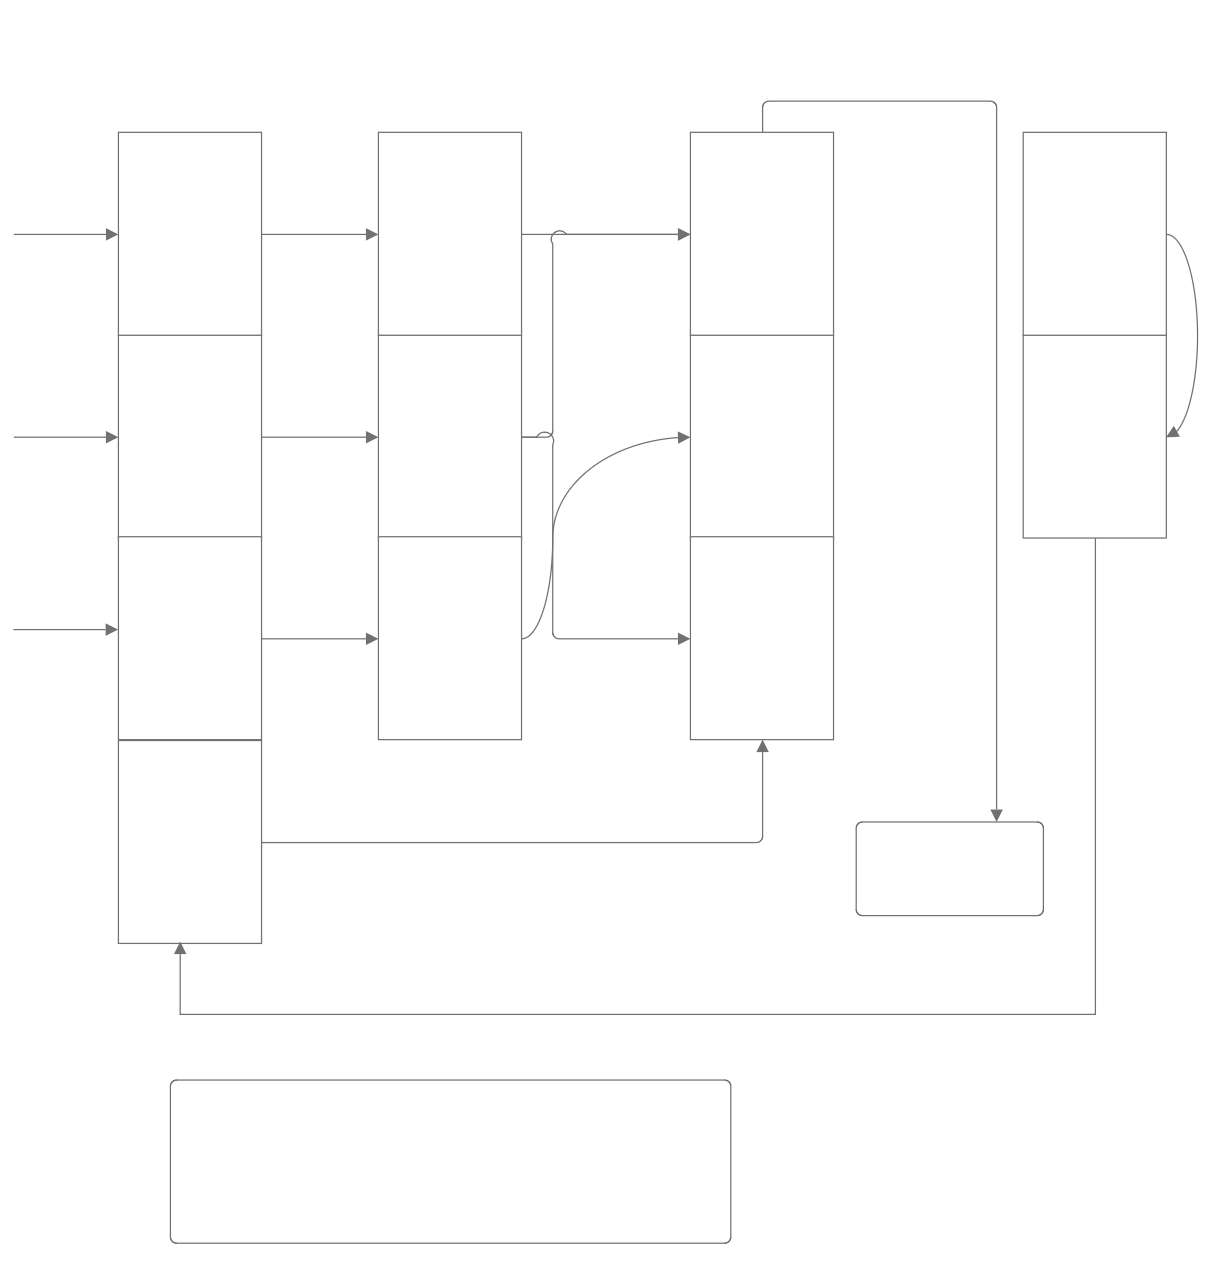
\includegraphics[width=0.5\linewidth]{schematic.png}
    \caption{Placeholder cable schematic}
    \label{fig:enter-label}
\end{figure}
\section{\label{sec:setup}Experimental Setup}
\subsection{Detector and instrumentation}
Here we give information about the detector set up and material: 3 plastic (carbon) scintillators. \blue{Maybe include details about the instrumentation used.}




\section{\label{sec:Results} Results}
\subsection{Thresholds and efficiency}
%%%%%%%%%%%%%%%%%%%%%%%%%%%%%%%%%%%%%%%%%%%%%%%%%%%%%%%%%%%%%%%%%%%%%%%%
\begin{acknowledgments}
\end{acknowledgments}

\bibliographystyle{apsrev4-2}
\begin{thebibliography}{99}

\bibitem{Ashkin1986}
A. Ashkin, J. M. Dziedzic, J. E. Bjorkholm, and S. Chu,
``Observation of a single-beam gradient force optical trap for dielectric particles,''
Opt. Lett. \textbf{11}, 288 (1986).

\bibitem{OpticalTweezerInstructions}
M. Prentiss, 
``Optical and Magnetic Tweezers: Advanced Physics Laboratory,''
Harvard Wiki (2003).

\bibitem{Smith1999AJP}
S. P. Smith et al.,
``Inexpensive optical tweezers for undergraduate laboratories,''
Am. J. Phys. \textbf{67}, 26--35 (1999).

% \bibitem{HoffmanPhysics191Writing}
% J. E. Hoffman,
% ``Hoffman-Physics191-Writing: Guidance on Scientific Paper Outline,''
% (2020). [Online: http://hoffman.physics.harvard.edu/]

\end{thebibliography}

\end{document}